\documentclass[a5paper]{article}
\usepackage[a5paper, top=8mm, bottom=8mm, left=8mm, right=8mm]{geometry}

\usepackage{polyglossia}
\setdefaultlanguage[babelshorthands=true]{russian}

\usepackage{fontspec}
\setmainfont{FreeSerif}
\newfontfamily{\russianfonttt}[Scale=0.7]{DejaVuSansMono}

\usepackage[font=scriptsize]{caption}

\usepackage{amsmath}
\usepackage{amssymb,amsfonts,textcomp}
\usepackage{color}
\usepackage{array}
\usepackage{hhline}
\usepackage{cite}

\usepackage[hang,multiple]{footmisc}
\renewcommand{\footnotelayout}{\raggedright}

\PassOptionsToPackage{hyphens}{url}\usepackage[xetex,linktocpage=true,plainpages=false,pdfpagelabels=false]{hyperref}
\hypersetup{colorlinks=true, linkcolor=blue, citecolor=blue, filecolor=blue, urlcolor=blue, pdftitle=1, pdfauthor=, pdfsubject=, pdfkeywords=}

\usepackage{tabu}

\usepackage{graphicx}
\usepackage{indentfirst}
\usepackage{multirow}
\usepackage{subfig}
\usepackage{footnote}
\usepackage{minted}
\usepackage{xcolor}

\newcommand{\attribution}[1] {
    \vspace{-5mm}\begin{flushright}\begin{scriptsize}\textcolor{gray}{\textcopyright\, #1}\end{scriptsize}\end{flushright}
}

\sloppy
\pagestyle{plain}

\title{Практика 14: REST-сервис}
\author{Юрий Литвинов\\\small{yurii.litvinov@gmail.com}}

\date{25.04.2022}

\begin{document}

\maketitle
\thispagestyle{empty}

\section{Краткий ликбез по веб-сервисам}

Веб-сервисы --- основные строительные блоки распределённых приложений и основной способ их интеграции. Веб-сервис запускается как отдельное приложение (или веб-приложение в рамках некоего веб-сервера, там он не отдельное приложение в общепринятом смысле, но close enough), слушает сетевые запросы и выдаёт ответы в каком-то из форматов сериализации. Реализуются они в целом так же, как и веб-приложения --- есть контроллеры, они обрабатывают запросы, десериализуя их параметры, работая при этом с моделью и, через модель, с данными. Концептуально простой веб-сервис устроен вот так:

\begin{center}
    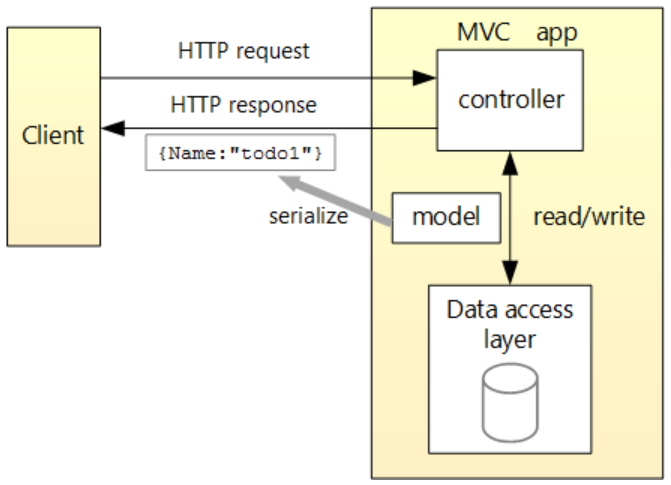
\includegraphics[width=0.4\textwidth]{webApiServiceDesign.png}
    \attribution{https://docs.microsoft.com/en-us/aspnet/core/tutorials/first-web-api}
\end{center}

Однако эта картинка несколько грешит против истины:

\begin{itemize}
    \item Схема с контроллерами используется, если сервис много чего умеет. В современных архитектурах сервисы стараются делать возможно более простыми, там полноценный MVC может быть оверкиллом. Тот же ASP.NET умеет <<минимальные>> веб-API, где можно декларативно отобразить URL каждого запроса в лямбда-функцию, которая его обрабатывает, так что весь сервис можно уместить в одном файле. У нас курс по архитектуре, поэтому я буду рекламировать более архитектурный подход.
    \item Дёргать прямо из контроллера Data Access Layer --- совершенно против идей предметно-ориентированного проектирования, и годится только для очень простых сервисов. Идеологически правильнее считать контроллер только <<средством доставки>>, задача которого --- принять запрос, десериализовать параметры и передать исполнение запроса доменной модели (причём в архитектурном стиле <<Ports and adapters>> и его производных даже на доменной модели, а адаптерам, которые верифицируют запрос и сконвертируют его в удобное для модели внутреннее представление).
    \item Моделью тут называется модель представления данных. Это вполне ок, но в реальности всё сложнее. Есть модель, которая <<Model>> в MVC, то есть обёртка над бизнес-логикой и слоем представления данных, <<бэкенд>> сервиса. Есть модель передачи данных, которая используется для сериализации-десериализации данных запроса. Может быть отдельно модель персистентности, которая нужна для удобства работы с базой (и, как правило, содержит в себе атрибуты, нужные для работы ORM-системы). В очень простых сервисах хоть все эти модели можно склеить в одну.
\end{itemize}

Конкретно в ASP.NET веб-сервис делается следующим образом:

\begin{itemize}
    \item Создаётся проект по шаблону <<ASP.NET Core Web API>>. Это на самом деле обычный ASP.NET, но без View и связанных с ним штук --- Razor, клиентских библиотек и т.п.
    \item Оставляются настройки по умолчанию, в частности, важно оставить галочку напротив поддержки OpenAPI (бывший Swagger). Эта штука нам потребуется для тестирования сервиса. В продакшене поддержку OpenAPI обычно убирают, но это легко делается правкой пары строк в Program.cs, поэтому при создании сервиса пусть будет. Ещё там установлена поддержка SSH --- потому что современные приложения работают только по защищённым протоколам передачи, и не установлена поддержка Docker --- как только вам про него расскажут, использование Docker станет обязательным, но всему своё время.
    \item В сгенерившемся по шаблону приложении есть один контроллер (WeatherForecastController.cs):
    \begin{itemize}
        \item Атрибут ApiController выставляет настройки по умолчанию для API, типа автоматического ответа HTTP 400 при провале валидации параметров запроса и т.п.
        \item Атрибут Route описывает, по какому URL доступны методы контроллера. Например, \verb|Route("[controller]")| делает контроллер доступным по чему-то вроде \url{https://localhost:8888/WeatherForecast}. GET-запрос по такому URL вызовет метод Get() контроллера.
        \item Логгер контроллеру для работы не нужен, но в реальной жизни логирование, конечно, активно используется.
    \end{itemize}
    \item В роли модели передачи данных в шаблоне используется класс WeatherForecast, обычный класс с public-свойствами. Таких моделей в одном сервисе может быть много, их обычно складывают в отдельную папку (по соглашению, Models).
    \item В Program.cs находится точка входа, которая конфигурирует приложение и которая запускает цикл обработки событий, слушающий сетевые запросы.
\end{itemize}

\section{Задача}

На практику будет задача одновременно на архитектуру и реализацию. Надо в командах по два человека спроектировать и реализовать REST-сервис, позволяющий интегрироваться с MyHwProj из домашней работы внешним системам.

Надо будет подумать над возможными запросами, описать модель данных и спроектировать REST API, как учили на лекции. При этом считаем, что потенциальные случаи использования нашего API такие:


\begin{itemize}
    \item Реализация внешнего клиента для студента или преподавателя
    \item Сервис, выполняющий агрегацию и анализ статистики по курсу
\end{itemize}

Поскольку вопросы сетевой безопасности мы ещё <<не проходили>>, авторизацию можно не делать. Опять-таки, API студентов и преподавателей могут быть разнесены по разным роутам. Реализацию бизнес-логики тоже можно пока не делать, сейчас наша задача --- именно спроектировать API и сделать веб-сервис, который бы позволил его тестировать/интегрироваться с ним. Поэтому можно симулировать реальные данные статическими полями с захардкоженной парой примеров.

Тестировать сервис, кстати, надо с использованием веб-интерфейса OpenAPI или, если ваша технология создания веб-сервисов OpenAPI не умеет, то SoapUI. Если на паре не успеете показать, опишите в README методику тестирования. Ещё чисто в учебных целях попробуйте выполнить какой-нибудь GET-запрос из браузера.

Кстати, можно использовать любой язык и любую технологию для реализации. Однако если хотите это сделать на .NET, может помочь туториал по веб-API \url{https://docs.microsoft.com/en-us/aspnet/core/tutorials/first-web-api} (только не увлекайтесь работой с базой данных). Задача предполагает чтение документации и самостоятельное разбирательство в деталях, поэтому и предполагается командная работа.

\end{document}
